% sesmesh — Solvent Excluded Surface meshes for molecules
% Copyright (c) 2026 Ugo Varetto
% SPDX-License-Identifier: MIT OR Apache-2.0

\section{Method}
\label{sec:method}

The algorithm follows one principle: the surface is defined by the exact
function~\eqref{eq:field}; discretization decides only \emph{where} it is
sampled, never \emph{what} is computed. Vertices are roots of $F$ on grid
edges and normals are its exact gradient. \Cref{fig:pipeline} shows the
pipeline.

\begin{figure}[t]
  \centering
  \begin{tikzpicture}[
      node distance=4mm and 4mm,
      box/.style={draw=black!60, rounded corners=2pt, fill=#1,
        align=center, font=\footnotesize, minimum height=11mm,
        text width=23mm, inner sep=2pt},
      box/.default=black!4,
      arr/.style={-{Latex[length=2mm]}, black!70}]
    \node[box] (in) {Structure file\\PDB, mmCIF,\\XYZ, PQR};
    \node[box, right=of in] (sel) {Selection,\\radii $\to$\\spheres};
    \node[box=blue!8, right=of sel] (arr) {SAS arrangement\\circles, exposed\\arcs, vertices};
    \node[box=blue!8, right=of arr] (cls) {Brick classifi-\\cation: touched,\\bounds, Lipschitz};
    \node[box=blue!8, below=of cls] (mesh) {Per surface brick:\\gather, SIMD field,\\MC, refinement};
    \node[box=blue!8, left=of mesh] (asm) {Global assembly\\prefix sums,\\edge references};
    \node[box=blue!8, left=of asm] (post) {Components,\\cavities,\\fragments};
    \node[box, left=of post] (out) {Smoothing,\\decimation;\\OBJ, PLY, MSMS};
    \draw[arr] (in) -- (sel); \draw[arr] (sel) -- (arr);
    \draw[arr] (arr) -- (cls); \draw[arr] (cls) -- (mesh);
    \draw[arr] (mesh) -- (asm); \draw[arr] (asm) -- (post);
    \draw[arr] (post) -- (out);
  \end{tikzpicture}
  \caption{Pipeline. Shaded stages form the surface core, which takes
    spheres and returns a mesh; parsing, radii and export are layers around
    it. Every stage after parsing runs in parallel and produces the same
    result for any number of threads.}
  \label{fig:pipeline}
\end{figure}

\subsection{The SAS arrangement}
\label{sec:arrangement}

All geometric constructions use 64-bit floating point. Spheres with
$R_i = 0$ are removed and exact duplicates (same centre within
$10^{-9}$\Ang{} and same radius) are collapsed. Spheres are sorted by the
Morton code of their cell for locality, and a uniform cell list with cell
size $2\max_i R_i$ (about 6.4\Ang{} for proteins with $r_p = 1.4$\Ang),
built by counting sort, answers range queries; very sparse inputs double the
cell size until the grid has at most $\max(65\,536, 8N)$ cells.

A sphere lying inside another is marked \emph{contained} and ignored.
For every intersecting pair $(i,j)$ a circle frame
$(\vect m, \vect u, \vect e_1, \vect e_2, \rho)$ is built. For each common
neighbour $k$, the points of circle $(i,j)$ inside ball $k$ form an angular
interval: with $\vect g = \vect m - \vect c_k$,
$\norm{\vect q(\theta) - \vect c_k}^2 = \norm{\vect g}^2 + \rho^2 +
2\rho(\cos\theta\, \vect e_1\cdot\vect g + \sin\theta\, \vect e_2\cdot\vect g)
< R_k^2$, i.e.\ $\cos(\theta - \varphi_k) < \beta_k$, which is empty, the
full circle, or an interval centred at $\varphi_k + \pi$. Endpoints are
computed as unit vectors with angle-addition formulas, and intervals are
sorted and merged on a monotone, trigonometry-free pseudo-angle; this made
the circle stage about $1.8\times$ faster on GroEL--GroES (PDB 1AON). A
circle covered completely is \emph{buried} and discarded; otherwise its
blockers $K(i,j)$ are the spheres with non-empty intervals. The endpoints of
exposed arcs are the SAS vertices---probe positions touching three atoms,
the vertices of the reduced surface of MSMS~\cite{sanner1996}. Each triple
$i < j < k$ is enumerated exactly once, from exposed circle $(i,j)$ and
blocker $k > j$, and kept if no other neighbour of $i$ contains it, a single
source of truth independent of how the arcs were merged. A sphere is
\emph{exposed} if it has no neighbour or at least one exposed circle; a
buried sphere still blocks but never yields a class-S candidate. Containment,
intersection and strict-inclusion tests use an absolute tolerance of
$10^{-9}$\Ang, which decides exactly fitting probes deterministically;
symmetric lattices, icosahedral and dodecahedral cages, collinear chains and
exact duplicates are covered by tests (\cref{sec:robustness}).

The cost is $O(N\bar k^2)$ for $\bar k$ neighbours per atom, dominated by
about 20 blocker tests for each of about 20 candidate circles per atom.
Single-threaded, the arrangement took 3.3\,ms for crambin (1CRN), 56\,ms for
haemoglobin (4HHB), 0.73\,s for 1AON (59\,k atoms) and 3.0\,s for the 80S
ribosome 4V6X (238\,k atoms) when it was first built; it now runs in
parallel per sphere.

\subsection{Sparse narrow-band brick lattice}
\label{sec:lattice}

\paragraph{Lattice and bricks.}
Samples lie on the lattice $\vect o + h\,(i,j,k)$, $i,j,k \in \mathbb Z$,
where the frame origin $\vect o$ is the centre of the bounding box rounded
to a multiple of $h$, so the lattice coincides with multiples of $h$ in
input coordinates and kernel coordinates stay small. A \emph{brick} is a
block of $B^3$ cells ($B = 10$ by default; it was measured 4--10\,\%
faster end to end than $B = 8$ on 4HHB and 1AON, while 4, 6, 14 and 16 were
slower). Each brick evaluates its own $(B+1)^3$ samples, an apron that
includes its upper faces, so bricks are independent work items; the
duplicated samples ($1.33\times$ at $B = 10$) buy freedom from
synchronization between bricks.

\paragraph{Clamped field.}
Exact values are needed only near the surface. With the band
$\delta = \sqrt3\,h$, \sesmesh{} evaluates
$\tilde F = r_p - \min\bigl(d(\vect x, P),\, r_p + \delta\bigr)$, which is
exact wherever $|F| \le \delta$, has the correct sign everywhere and is
still 1-Lipschitz. Distances beyond $D = r_p + \delta$ are never needed,
which bounds every candidate search.

\paragraph{Conservative classification.}
Let $\vect b$ be a brick centre, $\rho_b = \tfrac{\sqrt3}{2}Bh$ its
circumradius and $\varepsilon_c = 2\cdot10^{-3}$\Ang{} a margin above the
kernel's rounding error (\cref{sec:kernel}). Then:
\begin{enumerate}
  \item \emph{Touched set.} Bricks overlapping no ball
    $B(\vect c_i, R_i + \varepsilon_c)$ lie in $P$ and are uniformly
    outside; they are never enumerated. Every sphere marks the bricks it
    overlaps, in a dense bitset when the brick lattice has at most $2^{31}$
    bricks and by a parallel sort and deduplication of brick keys
    otherwise.
  \item \emph{Cheap bounds} from nearest-sphere queries:
    $s_{\mathrm{SAS}}(\vect b) \ge \rho_b + \varepsilon_c$ means the brick
    lies in $P$ (uniformly outside), and
    $s_{\mathrm{vdW}}(\vect b) \le -(\rho_b + \varepsilon_c)$ means it is
    uniformly inside, by~\ref{p:vdw}.
  \item \emph{Lipschitz test.} If
    $|\tilde F(\vect b)| > \rho_b + \varepsilon_c$, the brick is uniform
    with the sign of $\tilde F(\vect b)$, by~\ref{p:lipschitz}.
  \item Otherwise it is a \emph{surface brick}.
\end{enumerate}
Uniform bricks produce no geometry. This is the adaptive distance field
idea~\cite{frisken2000} and the brick culling of Hermosilla et
al.~\cite{hermosilla2017}, made exact by the Lipschitz bound. The same test
classifies the $2^3$ sub-blocks of each surface brick: samples that lie only
in uniform sub-blocks receive the value $\pm\delta$ (exact sign, inexact
value) without evaluation. Meshing needs exact values only at both ends of
sign-changing edges, which never touch a uniform sub-block, so this changes
no vertex. On 1AON about 23\,\% of samples are culled this way at
$h = 0.5$\Ang{} and about 56\,\% at $0.25$\Ang.

\paragraph{Candidate gathering.}
Candidates are gathered per active sub-block (centre $\vect b$,
circumradius $\rho$) within $G = r_p + \delta + \rho$ of $\vect b$ into
reusable thread-local structure-of-arrays buffers: the non-contained
spheres that can block (those that can contain a sample first, as only
they are scanned by the inside-SAS test), class-S candidates sorted by
distance (nearest first, for better pruning) with their blockers within
reach, class-C candidates with filtered blocker lists, and class-V
vertices within $G$. Any candidate that can be the closest point (at
distance $\le D$) of a sample in the sub-block lies within $G$ of
$\vect b$, and any sphere that can invalidate it contains a point within
$G$ of $\vect b$; the gathered sets therefore give the same minimum as the
global ones.

\subsection{Vectorized field kernel}
\label{sec:kernel}

SIMD lanes map to samples. The active samples of a sub-block are compacted
into 32-bit floating-point coordinate arrays, computed in the centred frame
from integer lattice indices and padded to a multiple of 16, so there is no
scalar tail. Vectors hold eight lanes (one AVX2 register, or two NEON
registers, which measured about 10\,\% faster than native four-lane NEON on
1AON thanks to the extra instruction-level parallelism). Per vector, the
kernel keeps the squared best distance, initialized to $D^2$, and processes
(1)~class-V vertices with one minimum per vertex; (2)~class-S candidates,
skipping a candidate when the lower bound
$\bigl|\norm{\vect x - \vect c} - R\bigr|$ improves no lane, otherwise
computing the candidate points, AND-reducing validity over the blockers
with an early exit once all active lanes are invalid, and updating the
minimum under a mask; (3)~class-C candidates in the same way. The output is
$\tilde F = r_p - \sqrt{\text{best}^2}$. On 4HHB at $h = 0.5$\Ang{} a
sub-block of $4^3$ cells evaluates about 96 samples against about 10
``inside'' spheres, 23 class-S candidates (19 blockers each), 41 class-C
candidates (11 blockers each) and 12 class-V vertices; validity tests
dominate.

\paragraph{Precision and seams.}
Kernel arithmetic is single precision in the centred frame. Differences of
nearby coordinates are exact (Sterbenz lemma), so the error is dominated
by input rounding, about $3\cdot10^{-5}$\Ang{} for coordinates up to
500\Ang{} from the origin; if any coordinate would lie more than 2\,000\Ang{}
from the frame origin, the engine evaluates samples with the exact
double-precision evaluator instead. Neighbouring bricks must agree on the
sign of every shared sample. An evaluated sample uses identical inputs in
every brick (position from integers, identical feature data, the same
instruction sequence and SIMD level, padded tails), every gathered set
contains all candidates that can win or invalidate, and skipping by lower
bound never changes the minimum, so evaluated values are bit-identical. A
sample that is sign-only in one brick has the exact sign, and the kernel's
error (below $10^{-4}$\Ang) is far below the classification margin
$\varepsilon_c$. Tests check every seam of random clusters and of crambin.

\subsection{Marching Cubes with a uniform face rule}
\label{sec:mc}

A lattice corner is \emph{inside} iff $\tilde F < 0$; zero counts as
outside, one rule everywhere. Cells are triangulated with a 256-case
Marching Cubes table~\cite{lorensen1987} whose ambiguous faces always
separate the inside corners. Because the rule depends only on the face,
adjacent cells agree on every shared face, which makes the output
crack-free, closed and edge-manifold. The table is generated by a
test-only program: per face, the rule gives oriented segments (inside on a
fixed side), which chain into loops per cell; each loop receives, among
\emph{all} its triangulations, one that (0)~has no diagonal joining two
vertices of the same cube face, since the neighbouring cell could produce
the same edge and four triangles would share it (this was found on 4HHB),
(1)~has no vertex whose area-weighted normal points from the outside end of
its edge to the inside end, (2)~has the least area (no folds) and (3)~has
the largest minimum angle. Tests check that the generator reproduces the
table, that every case uses exactly its crossing edges, that all
$3 \times 256 \times 16$ shared-face pairings match with opposite
orientations, that interior edges never lie in a face, and that the winding
is outward. Rows of cells without a sign change are skipped early, the
trimming idea of Flying Edges~\cite{schroeder2015}. The uniform rule does
not reproduce the topology of the trilinear interpolant in ambiguous cells
as MC33 does~\cite{lewiner2003,custodio2013}; it is chosen for guaranteed
manifoldness, and the topology converges as $h$ decreases.

\paragraph{Edge ownership.}
An edge is keyed by its lower sample and axis. A brick \emph{owns} the
edges whose lower sample lies in its half-open range $[0,B)^3$; edges on
its upper faces belong to the neighbours. A neighbour owning an edge with a
sign change is necessarily a surface brick, because a uniform brick has a
guaranteed uniform sign on its closed region, so cross-brick references
always resolve. The converse fails: a surface brick may own no crossing edge
and still contain crossing cells, whose crossings all lie on its upper
faces, so the cell pass runs for every surface brick (an early version
that skipped such bricks left holes).

\subsection{Exact vertices, analytic normals and attributes}
\label{sec:refine}

Each owned crossing edge, in ascending local edge order, creates one vertex.
Starting from the linear estimate $t_0 = \tilde F_a/(\tilde F_a - \tilde F_b)$,
the root of $g(t) = F(\vect a + t(\vect b - \vect a))$ is refined with a
safeguarded Newton iteration: the closest point of each evaluation gives
the exact gradient, of unit length, so one step from the linear guess
usually lands within tolerance; steps that leave the bracket fall back to
the Illinois method and then to bisection. With a tolerance of
$10^{-5}$\Ang{} and at most eight evaluations, refinement needs 2.2--2.5
field evaluations per vertex (pure Illinois needed 3.2--3.6). Evaluations
are scalar double precision against per-sub-block candidate lists whose
blockers are restricted to the spheres within reach; one evaluation costs
about 0.5\,\textmu s, about the SIMD kernel's cost per sample, so a
vectorized single-precision refinement would save little while losing
exact vertices.

The parameter is clamped to $t \in [10^{-4}, 1 - 10^{-4}]$ so that
vertices from edges meeting at a sample with $F \approx 0$ never coincide,
which excludes zero-area triangles; the induced error is at most
$10^{-4}h$. The clamp distance is also at least four single-precision ulps
of the largest coordinate, so the separation survives the 32-bit output
positions; it stays below $2.4\cdot10^{-4}$\Ang{} for coordinates up to
1\,000\Ang. (The ulp condition was added after a test 10\,000\Ang{} from
the origin collapsed two vertices into one 32-bit value.)

The final evaluation's closest point $\vect p$ gives the analytic normal
$\vect n = (\vect p - \vect v)/\norm{\vect p - \vect v}$ by~\ref{p:normal},
the patch type from the winning candidate class (S convex, C saddle, V
concave) and the nearest atom as the argmin of
$\norm{\vect v - \vect c} - r$ over the atoms generating that feature, the
``closest sphere'' semantics of MSMS~\cite{sanner1996}. For the SAS and vdW
surfaces the normal is the radial direction of the active sphere. A
cheaper \code{linear} mode skips refinement for previews.

\subsection{Deterministic global assembly}
\label{sec:assembly}

Each brick, in parallel, emits its triangles as references
(owning neighbour, local edge id) and stores its owned crossing edges as an
array sorted by edge id. A prefix sum of vertex counts over the sorted
brick list gives each brick's first global vertex; positions, normals and
attributes are concatenated in brick order; references are then resolved
in parallel by binary search in the owner's edge array. The output order
depends only on the brick order, the edge ids and the cell order, never on
scheduling. Every mesh is validated before it is returned---each undirected
edge used by exactly two triangles in opposite directions, no degenerate or
duplicate triangles, finite coordinates---and a violation is reported as an
internal error rather than written.

\subsection{Components, cavities and enclosure}
\label{sec:cavities}

Components are found by union--find over vertices along triangle edges.
Links always go from the larger root to the smaller, so the partition and
its labelling by smallest vertex index do not depend on the schedule even
with a lock-free parallel implementation. For each component, \sesmesh{}
computes in fixed-order double-precision sums the area, the signed volume
$\sum \vect v_0 \cdot (\vect v_1 \times \vect v_2)/6$, the Euler
characteristic $\chi = V - E + F$ and the genus $(2 - \chi)/2$.

Components with negative signed volume are cavities (\cref{sec:background}).
Three modes are offered: \code{keep} (the default: the exact SES including
cavities), \code{remove} (drop the cavities, as MSMS reports only the
external surface by default~\cite{msmsmanual}) and \code{only}. Removing a
cavity also removes every positive component inside it---a molecule
fragment enclosed in a pocket---found by a ray-parity point-in-mesh test of
one vertex after a bounding-box test. Filters by minimum cavity volume and
minimum component area apply in every mode. Triangles are reordered so that
each component is contiguous (for per-component groups in OBJ output).
Removing cavity components equals computing the SES of the unbounded
component of $P$ only, except in the degenerate case where a cavity's probe
balls touch external probe balls; both then belong to the same mesh
component and are kept.

\subsection{Sub-grid fragments}
\label{sec:fragments}

Where the solid side of the SES is a sheet thinner than $h$, Marching Cubes
can cut off small solid components that are not separate in the exact
surface. The typical case is two probe positions touching the same three
atoms from opposite sides of their plane, at a height just below $r_p$: the
SES spans the atom triangle with a sheet around a pinhole, its thickness
going to zero at the hole. In 4HHB at $h = 0.25$\Ang{} one such sheet
(atoms O1D of HEM~D148, OG of SER~D44 and CE2 of PHE~D45; probe height
1.371\Ang, pinhole radius 0.283\Ang) is 0.069\Ang{} thick at one lattice
node, where $F = -0.0049$\Ang, while its six neighbours are outside
($F = +0.025$ to $+0.219$\Ang); Marching Cubes emits an isolated octahedron
of 8 triangles and 0.037\AA$^2$ whose vertices are all concave. A flood
fill on a 0.01\Ang{} grid through $F < 0$ reaches the CE2 atom after
1.1\Ang: in the exact SES the sheet belongs to the main body.

Every true solid component contains an atom ball and its extreme points in
every direction lie on convex patches, so it has convex area of the order of
$4\pi R^2$. \sesmesh{} therefore defines a \emph{sub-grid fragment} as a
non-cavity component without any convex vertex; cavities contain a whole
probe ball (at least 11.5\AA$^3$ for $r_p = 1.4$\Ang) and are never
fragments. Fragments are dropped on request (\code{--drop-fragments}); the
option is off by default in the 1.x series so that default output stays
byte-identical to 1.0. \Cref{tab:fragments} shows that fragments are tiny
and well separated from the smallest true solid components. Finer grids
place more nodes in thin sheets (4HHB has 0, 2, 2, 1, 5 and 7 fragments at
$h = 0.5$, 0.35, 0.3, 0.25, 0.2 and 0.15\Ang) while each fragment's area
shrinks as $h^2$.

\begin{table}[t]
  \centering
  \caption{Sub-grid fragments in the validation corpus
    (\val{corpus-n} entries, Bondi radii, $r_p = 1.4$\Ang), counted with
    \sesmesh{} 1.1.0 (design document \S9.1). ``Triangles'' gives how many
    fragments have 8, 16, 24 or 32 triangles. On the \val{sweep-n}-entry
    sweep set at $h = 0.5$\Ang: 1\,026 fragments in 119 entries, the largest
    2.66\AA$^2$, the smallest true solid component 36.5\AA$^2$.}
  \label{tab:fragments}
  \small
  \begin{tabular}{@{}rrrlrr@{}}
    \toprule
    $h$ (\AA) & Fragments & Entries & Triangles 8/16/24/32 &
      Largest (\AA$^2$) & Smallest true solid (\AA$^2$) \\
    \midrule
    1.0  & 100   & 12 & 98/2/0/0       & 3.00 & 37.7 \\
    0.7  & 237   & 18 & 235/1/1/0      & 2.48 & 39.3 \\
    0.5  & 512   & 27 & 499/12/1/0     & 1.91 & 40.0 \\
    0.35 & 851   & 31 & 816/32/3/0     & 0.84 & 40.3 \\
    0.25 & 1\,358 & 36 & 1\,273/75/7/3 & 0.54 & 40.5 \\
    \bottomrule
  \end{tabular}
\end{table}

\subsection{Level of detail}
\label{sec:lod}

\paragraph{Spacing, presets and vertex density.}
The grid spacing $h$ is the primary control, with presets \code{draft}
(1.0\Ang), \code{low} (0.7\Ang), \code{medium} (0.5\Ang, the default, as in
ChimeraX~\cite{chimeraxsurface}), \code{high} (0.25\Ang) and \code{ultra}
(0.1\Ang). Users of MSMS think in vertices per \AA$^2$; for Marching Cubes
on a smooth surface with unit normal $\vect n$, the number of crossing
edges per unit area is about $(|n_x| + |n_y| + |n_z|)/h^2$, whose average
over uniformly distributed orientations is $1.5/h^2$. A requested density
$d$ is therefore mapped to $h = \sqrt{1.5/d}$; \cref{sec:density} confirms
the constant.

\paragraph{Smoothing with exact re-projection.}
Marching Cubes produces slivers where the surface nearly passes through
lattice nodes. Optional Taubin $\lambda|\mu$ smoothing~\cite{taubin1995}
($\lambda = 0.5$, $\mu = -0.53$, uniform umbrella Laplacian, parallel
Jacobi updates) is followed by re-projection of every vertex,
$\vect x \leftarrow \vect x - F(\vect x)\nabla F(\vect x)$, exact in one
step from inside $E$ by~\ref{p:project} (at most four steps), and by
recomputation of normals and attributes. In the tests, vertices stay within
$10^{-4}$\Ang{} of the SES after five rounds, the number of triangles with a
minimum angle below $10^\circ$ is more than halved and the area changes by
less than 1\,\%.

\paragraph{Decimation.}
Decimation uses Garland--Heckbert plane quadrics~\cite{garland1997} with
\emph{half-edge} collapses $u \to v$ only, so no new positions are created
and every retained vertex keeps its exact position, analytic normal, atom
and patch type. Instead of a global priority queue, each pass builds one
candidate per live edge (the cheaper direction, if its error is below the
bound), sorts the candidates in parallel with ties broken by vertex index
(so the result is deterministic) and applies them in order, skipping a
candidate whose endpoints' one-rings were already touched in that pass;
passes repeat until the target is met or nothing collapses. A collapse is
applied only if both endpoints share exactly two triangles, the link
condition holds, no triangle normal turns by more than about $78^\circ$, no
new triangle has a quality below 0.05 and the component keeps more than
four triangles. The mesh is then compacted and validated again. Crambin at
$h = 0.25$\Ang{} goes from 111\,076 to 27\,768 triangles in about 120\,ms;
on 1AON at 0.25\Ang{} the passes take about 6.5\,s where a heap with
re-queued edges took about 20\,s. Decimating a fine mesh concentrates
triangles where the surface bends (\cref{fig:lod}).

\begin{figure}[t]
  \centering
  \begin{subfigure}[b]{0.49\linewidth}
    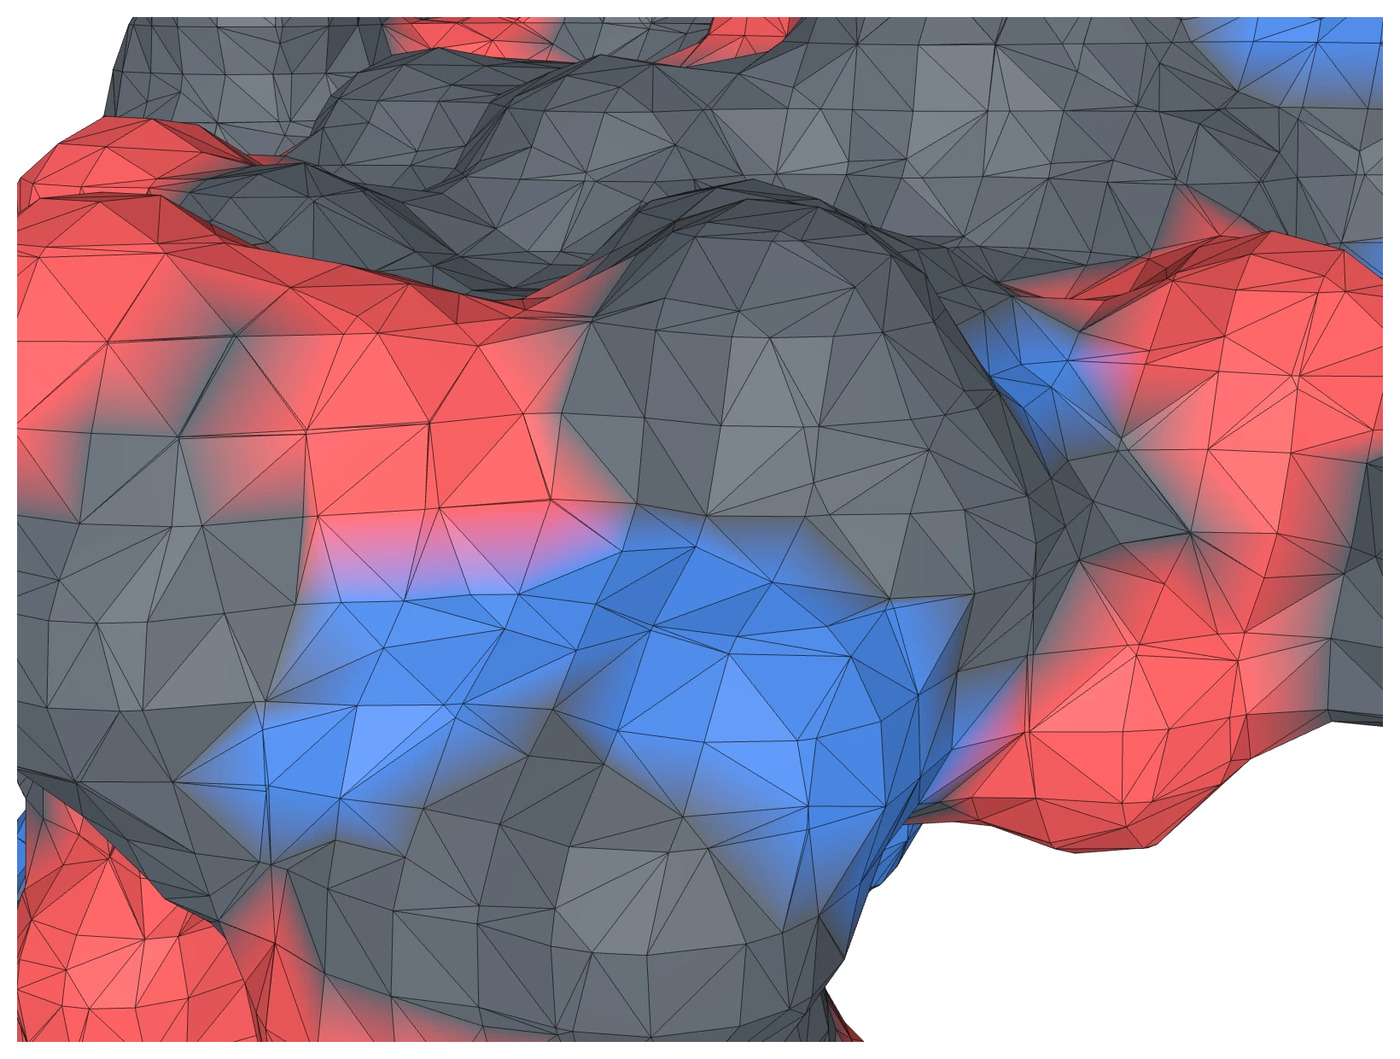
\includegraphics[width=\linewidth]{1crn-coarse}
    \caption{$h = 0.7$\Ang, 13\,996 triangles}
  \end{subfigure}\hfill
  \begin{subfigure}[b]{0.49\linewidth}
    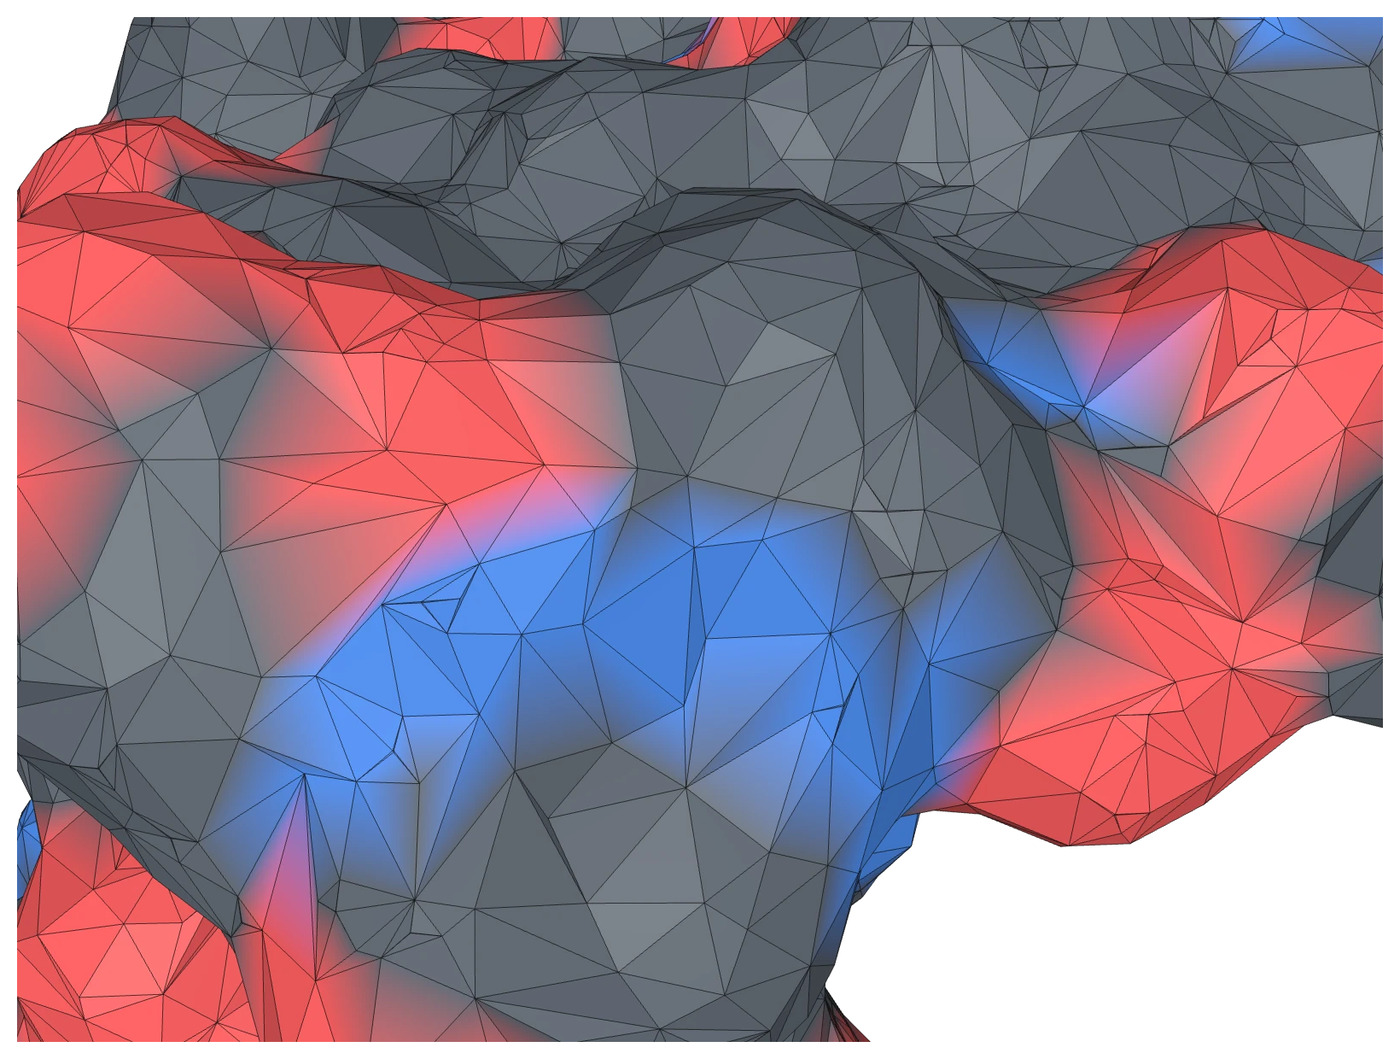
\includegraphics[width=\linewidth]{1crn-decimated}
    \caption{$h = 0.25$\Ang{} decimated to 13\,996 triangles}
  \end{subfigure}
  \caption{Two ways to spend the same triangle budget on crambin, coloured
    by element. (a)~A coarse grid gives uniform triangles everywhere.
    (b)~Decimating a fine mesh gives large triangles where the surface is
    flat and small ones where it bends; every vertex is still on the exact
    SES.}
  \label{fig:lod}
\end{figure}
